\section{Results}
\label{sec:results-v3}
SCIT-Speech used a shared index representation to combine low-rate speech reconstruction with receiver-side speaker identification. The central design was to transmit discrete codebook selections and reuse the recovered representation at the receiver. We evaluated this approach at a fixed three-layer residual vector quantization (RVQ) setting, $L=3$, with a nominal index rate of 1.5~kbit/s. The following results establish the representation and its learning stages, quantify the encoder resource savings, compare reconstruction with rate-matched codecs, and examine channel adaptation and speaker-information retention within the same index interface.

\subsection{A shared index representation supports reconstruction and receiver-side reuse}
\label{sec:rv3-payload}
The representation separates the information transmitted for each utterance from the model parameters stored at the two endpoints. A learned encoder converts mono 16-kHz speech into 1024-dimensional latent frames at 50~Hz~\cite{speechtokenizer}. Three residual quantizers successively encode each frame using three locally stored codebooks, each containing 1024 entries. At each quantization step, the selected codeword represents part of the residual left by the preceding steps. The channel then carries the three integer indices associated with each frame (Fig.~\ref{fig:rv3-components}a).

\begin{figure*}[t]
\centering
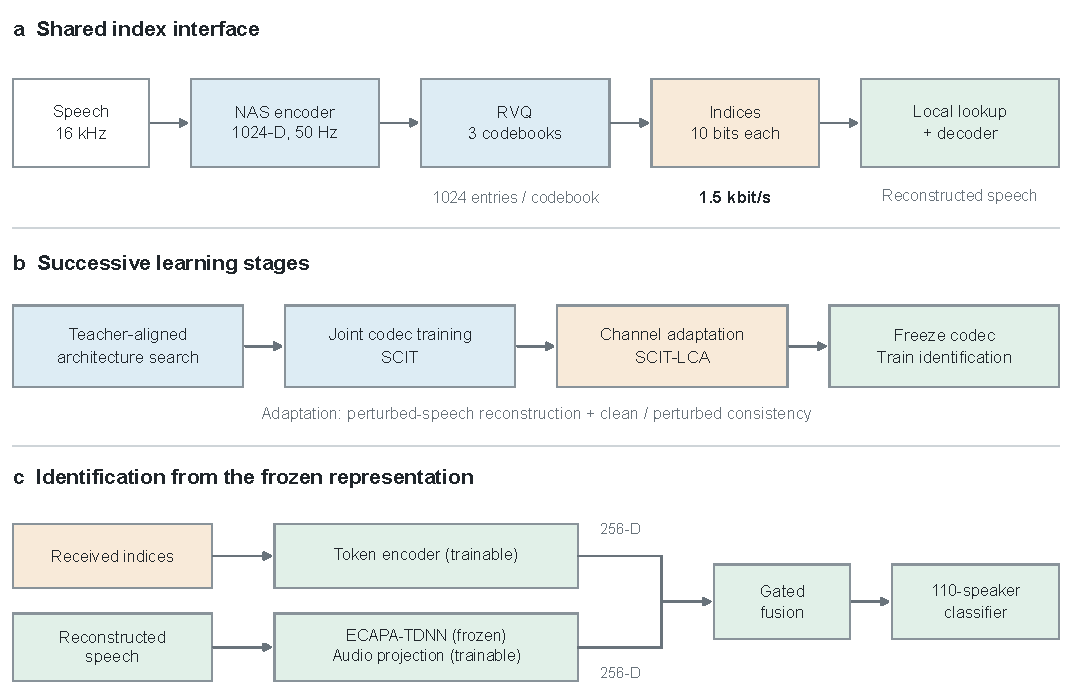
\includegraphics[width=\textwidth]{results_v3_assets/components.pdf}
\caption{Shared representation and learning stages of SCIT-Speech. \textbf{a}, The fixed $L=3$ interface maps speech to 50-Hz latent frames and transmits three 10-bit indices per frame. Local codebook lookup and summation provide the representation for waveform decoding. \textbf{b}, Teacher-aligned architecture search precedes joint codec training to obtain SCIT. Channel-aware fine-tuning produces SCIT-LCA, which is subsequently frozen for the identification study. The communication objective combines perturbed-speech reconstruction and clean--perturbed consistency. \textbf{c}, Receiver-side identification reads both the received indices and their reconstructed waveform. The token encoder, audio projection, fusion gate and classifier are trainable; the speech codec and ECAPA-TDNN backbone are frozen. Both branches produce 256-dimensional embeddings. No additional speaker embedding is transmitted.}
\label{fig:rv3-components}
\end{figure*}

This interface makes the bit budget explicit. With latent-frame rate $f_q=50$~Hz, codebook size $K=1024$ and $L=3$, each codebook selection requires ten bits:
\begin{equation}
\begin{aligned}
R_{\rm index}
&=Lf_q\lceil\log_2K\rceil\\
&=3\times50\times10=1500\ {\rm bit/s}.
\end{aligned}
\label{eq:rv3-rate}
\end{equation}
The resulting index stream is approximately 170.7 times smaller than 16-kHz, 16-bit mono pulse-code modulation (PCM), whose rate is 256~kbit/s. Throughout the comparisons, 1.5~kbit/s denotes this nominal index rate; packing and transport overhead are specified separately in Supplementary Methods S1. The 1024-dimensional codebook vectors remain local, so increasing the feature dimension does not require transmitting a continuous vector for every frame.

At the receiver, let $\widetilde I_{m,t}$ be the available index for quantizer $m$ and frame $t$, and let $C_m$ denote its codebook. The decoder reconstructs speech from the sum of the retrieved vectors:
\begin{equation}
\hat z_t=\sum_{m=1}^{3}C_m[\widetilde I_{m,t}],
\qquad \hat x=D_\phi(\hat Z).
\label{eq:rv3-reconstruction}
\end{equation}
This relation links the three evaluations below. Clean-channel reconstruction uses the original indices; robustness tests alter the indices supplied to the same lookup operation; and the speaker classifier reads both the received index sequence and the waveform reconstructed from it. The transmitted object remains unchanged across these receiver-side uses.

Learning proceeded in three stages after architecture selection (Fig.~\ref{fig:rv3-components}b). First, the encoder, codebooks and decoder were trained jointly to obtain the base codec, SCIT. Waveform and multi-scale mel reconstruction objectives were combined with adversarial, feature-matching and RVQ commitment losses. Frozen HuBERT features supervised the first quantizer~\cite{hubert}, providing a semantic learning signal alongside waveform reconstruction. Second, channel-aware fine-tuning produced SCIT-LCA using clean and perturbed index paths. Third, SCIT-LCA was frozen while a receiver-side classifier learned to identify speakers from its outputs.

These stages establish a common representation with distinct learning objectives. The base codec learns to reconstruct speech; channel adaptation trains reconstruction from perturbed indices; and the downstream classifier learns to read speaker information already present in the frozen representation. The transmitter continues to send only the three-layer index stream. The remaining sections evaluate the computational and task-level consequences of this design, beginning with the cost of generating the indices.

\subsection{Interface-preserving search reduces encoder resource requirements}
\label{sec:rv3-nas}
The encoder was optimized within a fixed latent interface so that computational cost could be reduced while retaining the 50-Hz, 1024-dimensional representation. Neural architecture search (NAS) varied width, stride arrangement, recurrent depth, activation and residual operators, with the overall downsampling factor held at 320. Candidate encoders therefore produced the same number and dimensionality of latent frames, allowing their outputs to be compared with a common pretrained SpeechTokenizer teacher~\cite{speechtokenizer}. The search operated on the encoder architecture, with the teacher's codebooks and decoder held fixed.

We profiled 8,192 configuration candidates and used successive teacher-alignment stages to select an architecture. The alignment objective combined latent distance, cosine agreement and temporal-difference matching. These terms compared feature values, directions and changes across adjacent frames, respectively. Candidate ranking combined alignment and reconstruction proxy scores with parameter count, multiply--accumulate operations (MACs) and real-time factor (RTF). The final architecture was selected by the combined score among nondominated candidates, coupling representation matching with resource efficiency. The complete search schedule is given in Methods and Supplementary Methods S2.

\begin{figure*}[t]
\centering
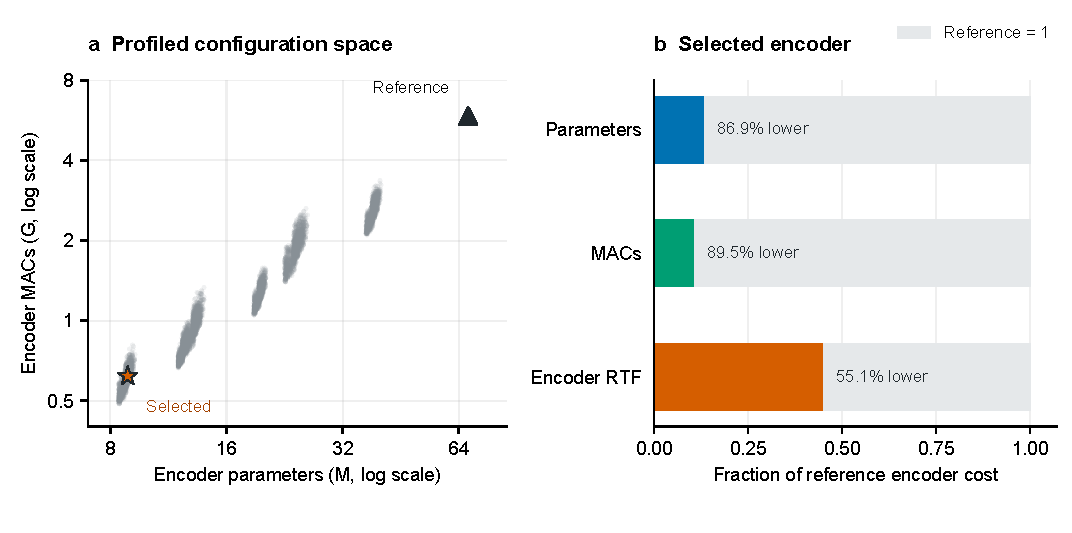
\includegraphics[width=\textwidth]{results_v3_assets/nas_resources.pdf}
\caption{Resource-efficient encoder selection at a fixed latent interface. \textbf{a}, Encoder parameter counts and MACs for 8,192 profiled configuration candidates. The triangle identifies the hand-designed reference and the star identifies the subsequently selected architecture. Both axes are logarithmic; each point represents a configuration profile. \textbf{b}, Selected-encoder resource requirements normalized to the reference. RTF was measured for encoder FP32 inference on an RTX 5070 Ti using a one-second input and averaging five synchronized passes.}
\label{fig:rv3-nas}
\end{figure*}

The selected encoder used a $(5,4,4,4)$ stride schedule, 24 initial filters, one bidirectional LSTM layer and Snake activation. Its parameter count was 8.873~M, compared with 67.706~M for the hand-designed reference, corresponding to an 86.9\% reduction. MACs decreased from 5.869~G to 0.618~G, a reduction of 89.5\% (Fig.~\ref{fig:rv3-nas}). These two measurements show that the selected architecture reduced both model size and arithmetic work at the preserved latent interface.

The corresponding encoder RTF decreased from 0.00819 to 0.00368 under the same profiling conditions, a reduction of 55.1\%. Thus, the resource savings were accompanied by faster measured encoder inference. Figure~\ref{fig:rv3-nas} places the selected architecture within the profiled configuration space and summarizes its costs relative to the reference. The reductions in parameters, MACs and measured inference time provide complementary evidence for a more economical speech encoder.

After selection, the NAS encoder, RVQ codebooks and decoder were trained jointly from scratch to obtain SCIT. Training used 27,039 LibriSpeech train-clean-100 utterances and a disjoint 1,500-utterance validation set~\cite{librispeech}; validation mel loss selected the retained checkpoint. This stage used HuBERT supervision of the first RVQ layer together with waveform reconstruction and adversarial learning. Search-time teacher alignment and subsequent codec learning therefore supported two successive steps: selecting the encoder architecture and training the complete speech representation.

Both SCIT and its channel-adapted variant retained the selected architecture and the three-layer transmission interface. The search consequently established a substantially smaller encoder that generated the same 1.5-kbit/s index payload. We next evaluated the speech reconstructed from this payload using external codecs at matched nominal rates.

\subsection{The 1.5-kbit/s codec improves objective reconstruction scores}
\label{sec:rv3-quality}
SCIT was compared with DAC and EnCodec at a nominal rate of 1.5~kbit/s on 300 LibriSpeech test-clean utterances. The evaluation used the first 300 entries in the retained manifest, processed each utterance in full and averaged metrics with equal utterance weights. The pretrained 16-kHz DAC model used three active quantizers~\cite{dac}. The pretrained 24-kHz EnCodec model used its 1.5-kbit/s setting~\cite{encodec}, with resampling before encoding and after decoding. Both external models were evaluated without fine-tuning on the comparison set.

\begin{table*}[t]
\centering
\caption{Clean-channel reconstruction on 300 LibriSpeech test-clean utterances. Entries are means [95\% utterance-bootstrap intervals]. The first three codecs share the nominal 1.5-kbit/s operating point; bold means identify the best in that group. Opus and PCM are higher-rate references. Lower mel-L1 and higher STOI/PESQ-WB are better.}
\label{tab:rv3-quality}
\small\setlength{\tabcolsep}{5pt}
\begin{tabular}{lrrrr}
\toprule
Codec & kbit/s & mel-L1 & STOI & PESQ-WB\\
\midrule
SCIT & 1.5 & \textbf{0.864} [0.855, 0.874] & \textbf{0.892} [0.889, 0.895] & \textbf{2.097} [2.067, 2.128]\\
DAC ($n_q=3$) & 1.5 & 1.232 [1.219, 1.245] & 0.799 [0.796, 0.803] & 1.284 [1.266, 1.303]\\
EnCodec & 1.5 & 1.282 [1.266, 1.297] & 0.848 [0.845, 0.851] & 1.612 [1.585, 1.638]\\
Opus & 6.0 & 2.302$^\dagger$ [2.275, 2.330] & 0.906 [0.903, 0.908] & 2.237 [2.187, 2.287]\\
PCM & 256 & 0.000 [0.000, 0.000] & 1.000 [1.000, 1.000] & 4.644 [4.644, 4.644]\\
\bottomrule
\end{tabular}
\par\smallskip
\parbox{\textwidth}{\footnotesize $^\dagger$Full-band mel-L1 is sensitive to low-rate Opus bandwidth reduction and is not a standalone cross-codec perceptual ranking. Intervals use 10,000 resamples and seed 42; displayed values are rounded to three decimals.}
\end{table*}


Three reference-based metrics characterized complementary aspects of reconstruction: log-mel spectral error (mel-L1), short-time objective intelligibility (STOI)~\cite{stoi}, and wideband perceptual evaluation of speech quality (PESQ-WB)~\cite{pesq}. All reconstructed signals were compared with their references at 16~kHz after trimming to their common length. The evaluation mel-L1 used a single-scale log-power representation, with its settings specified in Supplementary Methods S5. Table~\ref{tab:rv3-quality} reports the means and 95\% utterance-bootstrap intervals for each codec.

At the matched rate, SCIT achieved a STOI of 0.892, compared with 0.799 for DAC and 0.848 for EnCodec. The corresponding PESQ-WB scores were 2.097, 1.284 and 1.612. Thus, SCIT increased STOI by 0.093 and 0.044 over the two baselines, respectively, and increased PESQ-WB by 0.813 and 0.485 at the displayed precision. Spectral error followed the same ordering: SCIT obtained mel-L1 of 0.864, versus 1.232 for DAC and 1.282 for EnCodec.

\begin{table*}[t]
\centering
\caption{SCIT and SCIT-LCA on all 2,620 LibriSpeech test-clean utterances at $L=3$. Means are computed from paired utterances with matched perturbation seeds. Bold entries indicate the favourable direction within each condition, not statistical significance. Erasure and packet/burst masks use the previous original index, with the first frame protected.}
\label{tab:rv3-robustness}
\small\setlength{\tabcolsep}{6pt}
\begin{tabular}{lrrrrrr}
\toprule
& \multicolumn{2}{c}{mel-L1 $\downarrow$} & \multicolumn{2}{c}{STOI $\uparrow$} & \multicolumn{2}{c}{PESQ-WB $\uparrow$}\\
\cmidrule(lr){2-3}\cmidrule(lr){4-5}\cmidrule(lr){6-7}
Condition & SCIT & SCIT-LCA & SCIT & SCIT-LCA & SCIT & SCIT-LCA\\
\midrule
Clean & 0.9075 & \textbf{0.8711} & 0.8853 & \textbf{0.8922} & \textbf{1.9538} & 1.9397\\
10\% index erasure & 0.9986 & \textbf{0.9511} & 0.8457 & \textbf{0.8580} & 1.5364 & \textbf{1.5549}\\
3\% index substitution & 0.9716 & \textbf{0.9266} & 0.8640 & \textbf{0.8723} & 1.7027 & \textbf{1.7150}\\
5\% packet loss (100 ms) & 0.9336 & \textbf{0.8959} & 0.8727 & \textbf{0.8805} & \textbf{1.8096} & 1.8067\\
One 200-ms burst & 0.9271 & \textbf{0.8902} & 0.8752 & \textbf{0.8826} & \textbf{1.8674} & 1.8584\\
\bottomrule
\end{tabular}
\par\smallskip
\parbox{\textwidth}{\footnotesize The burst condition masks one randomly placed span of ten latent frames per utterance. All conditions use the token-domain protocol in Supplementary Methods S5.}
\end{table*}


The agreement across metrics is important because each measures a different aspect of the reconstructed signal. Lower mel-L1 indicates closer spectral reconstruction, while higher STOI and PESQ-WB indicate better objective intelligibility and perceptual-quality estimates. SCIT led the evaluated matched-rate settings on all three quantities. Its 95\% utterance-bootstrap intervals were also separated from those of both baselines for each metric, supporting the consistency of the observed ordering over this evaluation set.

The higher-rate Opus reference provided a complementary bitrate comparison. At a requested 6~kbit/s, Opus achieved STOI of 0.906 and PESQ-WB of 2.237. SCIT reached STOI within 0.014 of this reference using one quarter of its nominal bitrate, with PESQ-WB of 2.097. PCM passthrough at 256~kbit/s supplied the uncompressed reference. These comparisons locate the 1.5-kbit/s operating point relative to both learned codecs at the same rate and conventional coding at a higher rate.

For Opus, full-band mel-L1 was higher despite its higher STOI and PESQ-WB; the spectral metric is sensitive to bandwidth reduction at low coding rates. We therefore read the spectral and perceptual measures together. Across the matched-rate neural codecs, their agreement supports the reconstruction capability of the shared index representation. Having established its clean-channel performance, we next examined whether channel-aware learning improved reconstruction when some received indices were altered.

\subsection{Channel adaptation improves reconstruction from perturbed indices}
\label{sec:rv3-robustness}
An index error changes the codeword supplied to the decoder and therefore changes the reconstructed latent frame. SCIT-LCA addressed this perturbation at the representation interface by fine-tuning SCIT with clean and corrupted index paths. The communication branch sampled clean transmission, 5\% or 10\% index erasure, or 1\% or 3\% index substitution, alongside training-time RVQ-depth sampling. The architecture and codebook sizes were retained, and every evaluation reported here used the fixed $L=3$ operating point.

The adaptation objective linked reconstruction of the source signal to agreement between clean and perturbed decodes. For the original waveform $x$, clean decode $\hat{x}_{L}^{\,c}$ and perturbed decode $\hat{x}_{L}^{\,p}$, the implemented objective was
\begin{equation}
\begin{split}
\mathcal L_{\rm LCA}
=\mathcal L_{\rm base}
+1.5\bigl[&
500\mathcal L_{\rm wav}(x,\hat{x}_{L}^{\,p})\\
&+\mathcal L_{\rm mel}^{\rm ms}(x,\hat{x}_{L}^{\,p})
+0.5\mathcal L_{\rm cons}\bigr],
\end{split}
\label{eq:rv3-lca}
\end{equation}
where $\mathcal L_{\rm cons}$ is the multi-scale mel distance between the clean and perturbed decodes. The source-reconstruction terms train the perturbed path to recover the utterance, while consistency aligns its output with the corresponding clean reconstruction. The communication terms trained the decoder, alongside the full-depth branch's encoder and quantizer objectives. Validation communication-branch mel loss selected the SCIT-LCA checkpoint; full implementation details are given in Methods and Supplementary Methods S4.

We compared SCIT and SCIT-LCA on all 2,620 LibriSpeech test-clean utterances using matched utterances and perturbation seeds (Table~\ref{tab:rv3-robustness}). The test conditions comprised clean transmission, independent index errors and temporally grouped masks. Independent errors corresponded to perturbations included during fine-tuning, whereas packet and burst masks tested additional temporal patterns. The full-set evaluation complements the 300-utterance external-codec comparison with a direct, paired assessment of channel adaptation.

SCIT-LCA improved mel-L1 and STOI in every reported condition. On clean speech, mel-L1 decreased from 0.9075 to 0.8711 and STOI increased from 0.8853 to 0.8922. Under 10\% index erasure, mel-L1 decreased from 0.9986 to 0.9511 and STOI increased from 0.8457 to 0.8580. The corresponding adaptation gains were larger under erasure than under clean transmission: mel-L1 decreased by 0.0475 rather than 0.0364, and STOI increased by 0.0123 rather than 0.0069.

The independent-error conditions also showed higher PESQ-WB after adaptation. At 10\% erasure, PESQ-WB increased from 1.5364 to 1.5549. At 3\% substitution, SCIT-LCA improved all three metrics, reducing mel-L1 by 0.0451 and increasing STOI and PESQ-WB by 0.0082 and 0.0122, respectively. These results show a consistent improvement across the spectral, intelligibility and perceptual-quality measures for the two tested independent-index perturbations.

\begin{table*}[t]
\centering
\caption{Closed-set speaker identification from a frozen SCIT-LCA payload ($L=3$, 110 speakers, 1,650 test utterance groups). All entries are percentages. Mean $\pm$ SD uses the sample standard deviation across three training seeds. Worst 10\% is the mean accuracy of the 11 lowest-accuracy speakers. The last column reports within-seed hierarchical-bootstrap intervals.}
\label{tab:rv3-speaker}
\small\setlength{\tabcolsep}{5pt}
\begin{tabular}{lrrrrrr}
\toprule
Seed & Top-1 & Macro-F1 & Top-5 & ECE & Worst 10\% & Top-1 95\% CI\\
\midrule
41 & 95.03 & 94.94 & 99.39 & 1.30 & 76.97 & [93.21, 96.73]\\
42 (delivery) & 94.18 & 94.14 & 99.27 & 2.04 & 73.94 & [92.12, 95.88]\\
43 & 95.58 & 95.56 & 99.39 & 1.92 & 82.42 & [94.00, 97.03]\\
\textbf{Mean} & \textbf{94.93 $\pm$ 0.70} & \textbf{94.88 $\pm$ 0.71} & \textbf{99.35} & \textbf{1.75} & \textbf{77.78} & --\\
\bottomrule
\end{tabular}
\par\smallskip
\parbox{\textwidth}{\footnotesize Seed 42 was predeclared for delivery. Intervals are retained from the archived hierarchical-bootstrap analysis; execution metadata and its author-confirmation item are documented in Methods and Supplementary Methods S7.}
\end{table*}


To examine temporally grouped errors, the packet condition masked five-frame groups, corresponding to 100~ms, with probability 5\%; the burst condition masked one randomly positioned ten-frame span, corresponding to 200~ms, per utterance. Masked positions used the preceding original index, with the first frame protected, following the token-domain protocol in Supplementary Methods S5. SCIT-LCA increased STOI from 0.8727 to 0.8805 for packet masks and from 0.8752 to 0.8826 for burst masks. Mel-L1 decreased from 0.9336 to 0.8959 and from 0.9271 to 0.8902, respectively.

PESQ-WB showed a smaller, condition-dependent response: it decreased by 0.0141 under clean transmission and by 0.0030 and 0.0090 under packet and burst masks. Thus, the broadest adaptation benefit was the joint improvement in spectral error and STOI, with an additional PESQ-WB gain under independent index errors. Channel-aware learning extended the utility of the same low-rate representation across the evaluated perturbation patterns while preserving its transmission format.

\subsection{A frozen index representation retains speaker information}
\label{sec:rv3-speaker}
We next asked whether the representation learned for speech reconstruction also retained information useful for identifying the speaker. SCIT-LCA was frozen at $L=3$, and its index sequences and reconstructed waveforms were cached before classifier training. The receiver therefore learned to read a fixed speech representation. The codec continued to operate at 1.5~kbit/s, while the additional learning took place in the receiver-side identification module.

Two complementary views of the representation were available to this module (Fig.~\ref{fig:rv3-components}c). The token branch embedded the three index sequences and processed them with temporal residual blocks and attentive statistics pooling, producing a 256-dimensional embedding. The audio branch applied pretrained ECAPA-TDNN~\cite{ecapa} to the matching reconstruction and projected its output to the same dimension. An element-wise gate combined the two embeddings, and additive angular-margin objectives trained the fusion and auxiliary branch heads~\cite{arcface}. Test predictions used the fusion head. The speech codec and ECAPA backbone remained frozen; the token encoder, audio projection, gate and classification heads were trainable.

This arrangement places the two descriptions of the utterance at the receiver. The token branch reads discrete codeword selections, whereas the audio branch reads the waveform obtained by decoding those selections. Both inputs originate from the same transmitted indices, and their time windows were matched during training and evaluation. The design consequently adds receiver-side analysis while maintaining the original speech payload.

The closed-set evaluation used 110 speakers from the microphone-1 recordings of VCTK 0.92~\cite{vctk}. Each speaker contributed 80, 15 and 15 utterance groups to training, validation and test, respectively, yielding 8,800 training, 1,650 validation and 1,650 test items. Utterance groups were disjoint across splits, with the same enrolled identities represented in each split. Matched token and audio crops covered up to three seconds, and validation and test used deterministic centre crops with all three RVQ layers.

Three training runs used seeds 41, 42 and 43 under the same fixed split. Validation macro-F1 selected checkpoints, and validation data fitted a scalar temperature for probability calibration. Each configuration was then evaluated once on the locked test set. This procedure kept model selection and calibration separate from final measurement, while the three runs measured variation arising from classifier training. Detailed optimization and statistical procedures are provided in Methods and Supplementary Methods S6--S7.

\balance
Mean Top-1 accuracy reached $94.93\%\pm0.70\%$ and mean macro-F1 reached $94.88\%\pm0.71\%$, where the variation is the sample standard deviation across the three training seeds (Table~\ref{tab:rv3-speaker}). Mean Top-5 accuracy was 99.35\%. Individual Top-1 accuracies ranged from 94.18\% to 95.58\%, and the closely corresponding macro-F1 values show that the aggregate result was also reflected in the class-balanced score.

The table additionally reports within-seed hierarchical-bootstrap intervals, obtained by resampling speakers and then utterance groups within speakers. The lowest of the three interval endpoints was 92.12\%. Expected calibration error averaged 1.75\% after validation-only temperature fitting. The mean accuracy of the lowest-performing 10\% of speakers was 77.78\%, providing a complementary view of variation across identities alongside the overall accuracy.

These results show that the frozen three-layer representation retained speaker information that could be recovered with high accuracy across the 110 enrolled identities. Because both classifier inputs were derived from the received indices, identification required no additional transmitted identity vector. Receiver-side reuse thus extended the role of the low-rate payload from waveform reconstruction to speaker identification while leaving the speech codec unchanged.
